\documentclass{article}

\usepackage[utf8]{inputenc}
\usepackage[brazil]{babel}
\usepackage{amsmath, amssymb}
\usepackage{graphicx}
\usepackage{hyperref}
\usepackage{geometry}
\usepackage{caption}
\usepackage{pgffor}

\geometry{margin=1in}
\graphicspath{{imagens/}}

\title{Representações Não Lineares}
\author{Eduardo Henrique Basilio de Carvalho}
\date{\today}

\begin{document}

\maketitle

\section*{Questão 1}

\ref{fig:resposta_oscilador} mostra a resposta do oscilador de Van der Pol para condições iniciais $y(0) = 0$ e entrada

\begin{equation}
    u(t) = A \cdot \frac{1}{M} \sum_{k=1}^{N} c_k \sin\left(2\pi f_k t + \phi_k\right)    
\end{equation}
com $A = 1.0$, $M = 100$, $N = 100$, $c_k$ definidos aleatoriamente, $f_k$ variando de $0.2$ a $60.0$ Hz, duração de $60.0$ s e passo de integração $dt = 0.001$ s.

\begin{figure}
    \centering
    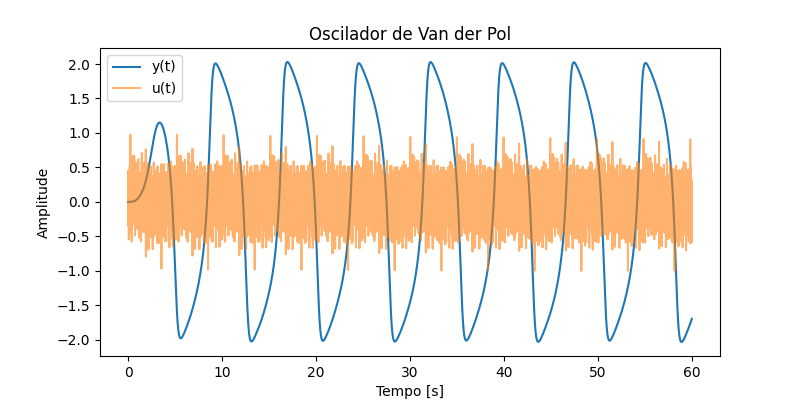
\includegraphics[width=\textwidth]{resposta_oscilador.png}
    \caption{Resposta do oscilador de Van der Pol à entrada $u(t)$.}
    \label{fig:resposta_oscilador}
\end{figure}

\subsection*{a}

Com a representação em série de Volterra, uma estimativa inadequada é esperada. A representação em série de Volterra funciona bem para sistemas fracamente não lineares e com “memória evanescente”. No entanto, o oscilador de Van der Pol é um sistema auto-oscilatório que possui um ciclo limite, não a propriedade de memória evanescente em torno de sua origem instável. Com uma amplitude de entrada de 1, uma abordagem de Volterra padrão (invariante no tempo e centrada em zero) tende a ser imprecisa. Seria mais apropriado, embora mais complexo, modelar as perturbações em torno do próprio ciclo limite usando uma abordagem de Volterra variante no tempo. \ref{aproximacao_volterra} mostra a comparação entre a resposta real do sistema e a resposta estimada usando uma aproximação de Volterra de segunda ordem.

\begin{figure}
    \centering
    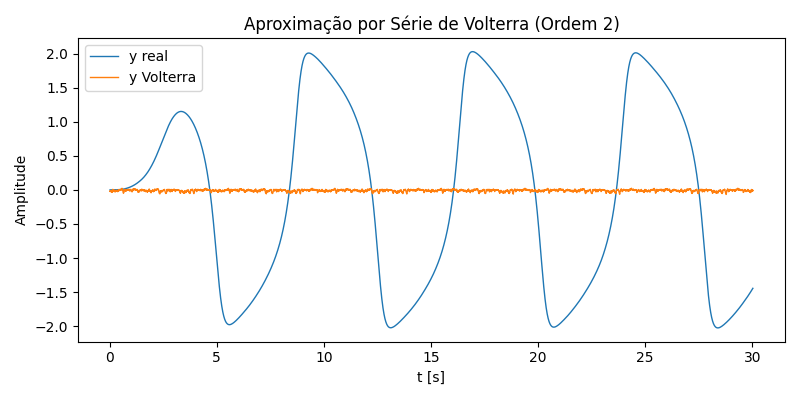
\includegraphics[width=\textwidth]{aproximacao_volterra.png}
    \caption{Comparação entre a resposta real do sistema e a resposta estimada usando uma aproximação de Volterra de segunda ordem.}
    \label{aproximacao_volterra}
\end{figure}

\subsection*{b}

A representação de Hammerstein geralmente não é adequada. Um modelo de Hammerstein presume uma estrutura em que a não linearidade estática atua apenas na entrada, seguida por um bloco de dinâmica linear $(u \rightarrow g(\cdot) \rightarrow L(s) \rightarrow y)$. O oscilador de Van der Pol viola fundamentalmente essa suposição, já que sua não linearidade é interna e dependente do estado (o termo de amortecimento depende de $y$ e $\dot{y}$), e não uma simples transformação estática da entrada $u$. Além disso, o sistema é um auto-oscilador com um ciclo limite, o que entra em conflito com a premissa de que a dinâmica (após a não linearidade) é linear e possui memória evanescente. Por causa dessa incompatibilidade estrutural, o método de testes desacoplados provavelmente falha em encontrar um modelo válido, pois a resposta do sistema depende crucialmente de seu estado interno (como a fase no ciclo limite), algo que uma transformação estática $g(u)$ não consegue capturar. \ref{aproximacao_hammerstein} mostra a comparação entre a resposta real do sistema e a resposta estimada usando uma aproximação de Hammerstein obtida por testes desacoplados.

\begin{figure}
    \centering
    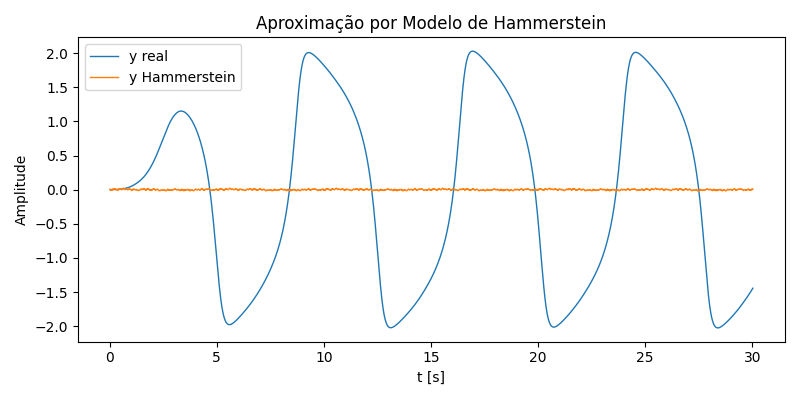
\includegraphics[width=\textwidth]{aproximacao_hammerstein.png}
    \caption{Comparação entre a resposta real do sistema e a resposta estimada usando uma aproximação de Hammerstein.}
    \label{aproximacao_hammerstein}
\end{figure}

\subsection*{c}

Um modelo de Wiener, que assume que toda a não linearidade do sistema pode ser representada por um mapa estático $g(\cdot)$ aplicado após um bloco de dinâmica linear $u \rightarrow L(s) \rightarrow w \rightarrow g(\cdot) \rightarrow y$, também não é bom candidato para representar este sistema. O oscilador de Van der Pol conflita diretamente com essa estrutura, já que sua não linearidade é interna e dependente do estado (o termo de amortecimento $(1-y^2)\dot{y}$), e não uma simples distorção estática da saída de um filtro linear. Adicionalmente, o sistema possui um ciclo limite auto-oscilatório, introduzindo uma memória de fase e dinâmicas internas que a estrutura Wiener (LTI + mapa estático) não consegue capturar. Portanto, é muito provável que os testes desacoplados falhem em encontrar um modelo válido devido a essa incompatibilidade estrutural fundamental. \ref{aproximacao_wiener} mostra a comparação entre a resposta real do sistema e a resposta estimada usando uma aproximação de Wiener obtida por testes desacoplados.

\begin{figure}
    \centering
    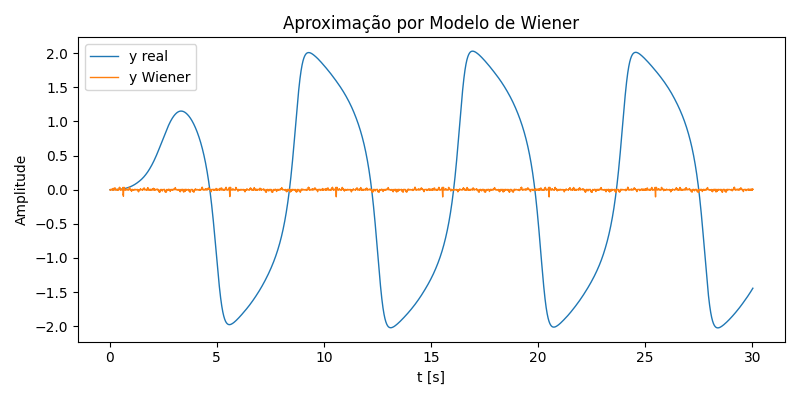
\includegraphics[width=\textwidth]{aproximacao_wiener.png}
    \caption{Comparação entre a resposta real do sistema e a resposta estimada usando uma aproximação de Wiener.}
    \label{aproximacao_wiener}
\end{figure}

\subsection*{d}

Um modelo NARX é uma escolha razoável e substancialmente mais flexível do que as estruturas Wiener ou Hammerstein para este sistema. A principal vantagem do NARX é usar tanto entradas passadas ($u(t-k)$) quanto saídas passadas ($y(t-k)$) como regressores, o que permite capturar dinâmicas complexas dependentes do estado. Isso é ideal para o oscilador de Van der Pol, cuja não linearidade (o amortecimento dependente do estado) é interna. \ref{aproximacao_narx} mostra a comparação entre a resposta real do sistema e a resposta estimada usando uma aproximação NARX.

\begin{figure}
    \centering
    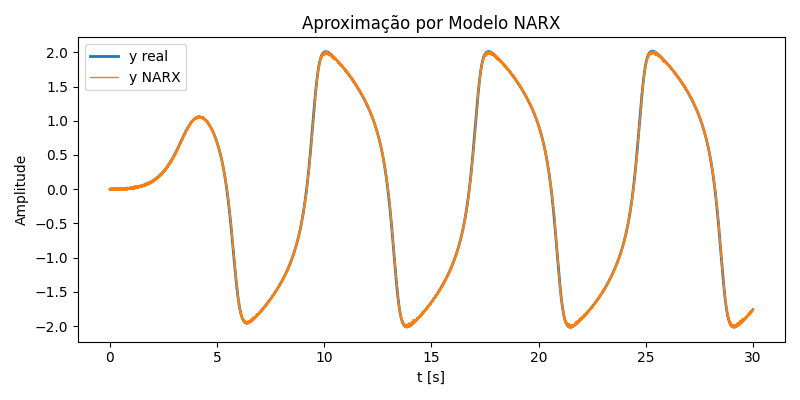
\includegraphics[width=\textwidth]{aproximacao_narx.png}
    \caption{Comparação entre a resposta real do sistema e a resposta estimada usando uma aproximação NARX.}
    \label{aproximacao_narx}
\end{figure}

\ref{fig:aproximacao_narx_teste} valida a generalização do modelo NARX em um conjunto de dados de teste diferente do conjunto de treinamento.

\begin{figure}
    \centering
    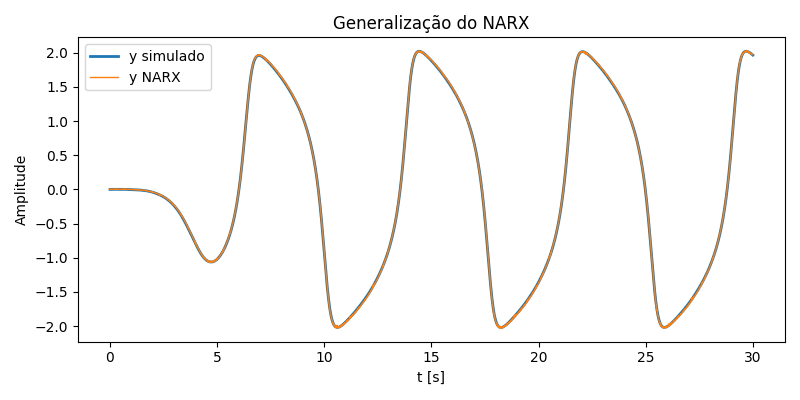
\includegraphics[width=\textwidth]{aproximacao_narx_teste.png}
    \caption{Validação da generalização do modelo NARX em um conjunto de dados de teste.}
    \label{fig:aproximacao_narx_teste}
\end{figure}

\section*{Questão 2}

\subsection*{a}

Para estimar a saída do sistema de resfriamento, séries de Volterra com graus de 1 a 3 foram testadas. Além da estimação sobre os dados brutos, também foi testada a estimação sobre os dados com a média subtraída e com média móvel, em janela de 10 \% da duração total, subtraída. Os parâmetros $a$, $M$ e $\alpha$ foram otimizados por busca em grade. \ref{fig:volterra_1_raw} a \ref{fig:volterra_3_remmvavg} mostram as melhores aproximações encontradas para cada grau e pré-processamento.

\foreach \order in {1,2,3} {
    \foreach \preprocess in {raw, remmean, remmvavg} {
        \begin{figure}
            \centering
            \includegraphics[width=\textwidth]{volterra_\order_\preprocess.png}
            \caption{Aproximação de Volterra de grau \order\ com pré-processamento \preprocess.}
            \label{fig:volterra_\order_\preprocess}
        \end{figure}
    }
}

Pelas curvas, nenhum dos modelos conseguiu capturar adequadamente o comportamento do sistema. A melhor aproximação foi a de grau 3 com remoção da média móvel, com erros ainda significativos.

\subsection*{b}

A estimação dos estados por \textbf{Takagi-Sugeno} usa o modelo

\begin{equation}
x_{k+1} = \sum_{r=1}^{R} \mu_r(x_k, u_k) \left( A_r x_k + B_r u_k + c_r \right)
\end{equation}

onde $\mu_r(x_k, u_k)$ é a função de pertinência da regra $r$ baseada no estado atual $x_k$ e entrada $u_k$, $A_r$ é a matriz de dinâmica local, $B_r$ é o vetor de ganho de entrada local, $c_r$ é o termo de offset local, e $R$ é o número de regras. Tais parâmetros foram otimizados por busca em grade. As estimações sobre conjunto de treinamento e teste são mostradas em \ref{fig:comparacao_treino} e \ref{fig:comparacao_teste}, respectivamente.

\begin{figure}
    \centering
    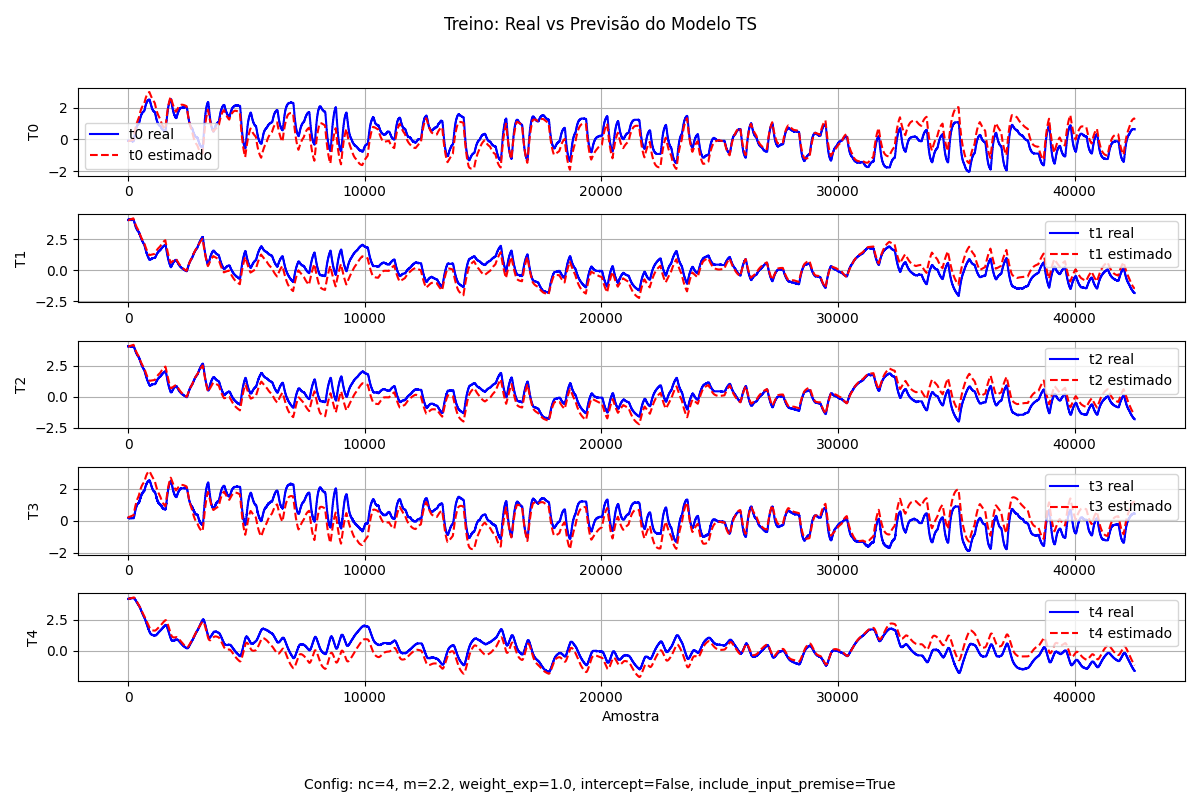
\includegraphics[width=\textwidth]{comparacao_treino.png}
    \caption{Comparação entre a saída real e estimada do sistema de resfriamento no conjunto de treinamento.}
    \label{fig:comparacao_treino}
\end{figure}

\begin{figure}
    \centering
    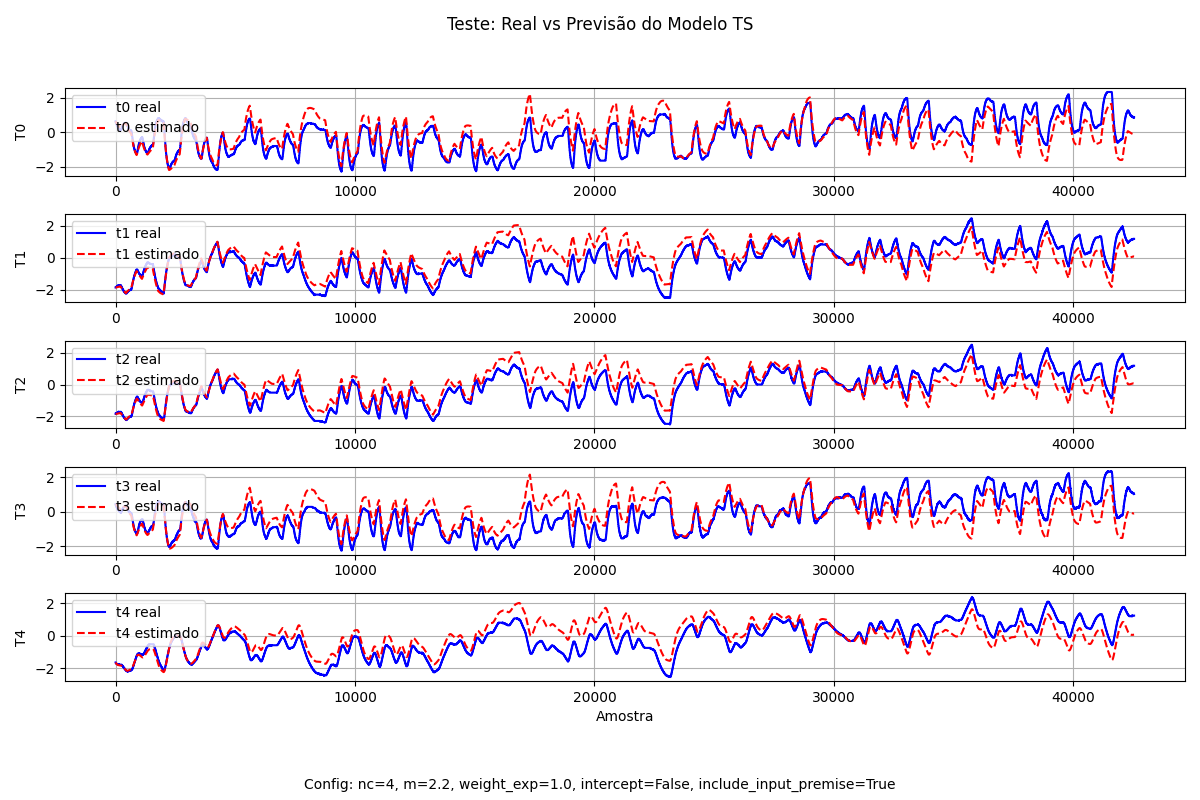
\includegraphics[width=\textwidth]{comparacao_teste.png}
    \caption{Comparação entre a saída real e estimada do sistema de resfriamento no conjunto de teste.}
    \label{fig:comparacao_teste}
\end{figure}

\end{document}